% Additional illustration 1: method overview (candidate Fig. 1, §3.1).
% Workers feed arrivals into an append-only history log; the propagator call is
% a pure function of that log and emits one candidate; a second branch replays
% the same log into the reported estimator.
\documentclass[tikz,border=4pt]{standalone}
\usepackage{newtxtext,newtxmath}
\usepackage{amsmath}
\usetikzlibrary{arrows.meta,positioning,calc,fit,shapes.misc}
\definecolor{async}{HTML}{0072B2}
\definecolor{sync}{HTML}{D55E00}
\definecolor{reject}{HTML}{009E73}

\begin{document}
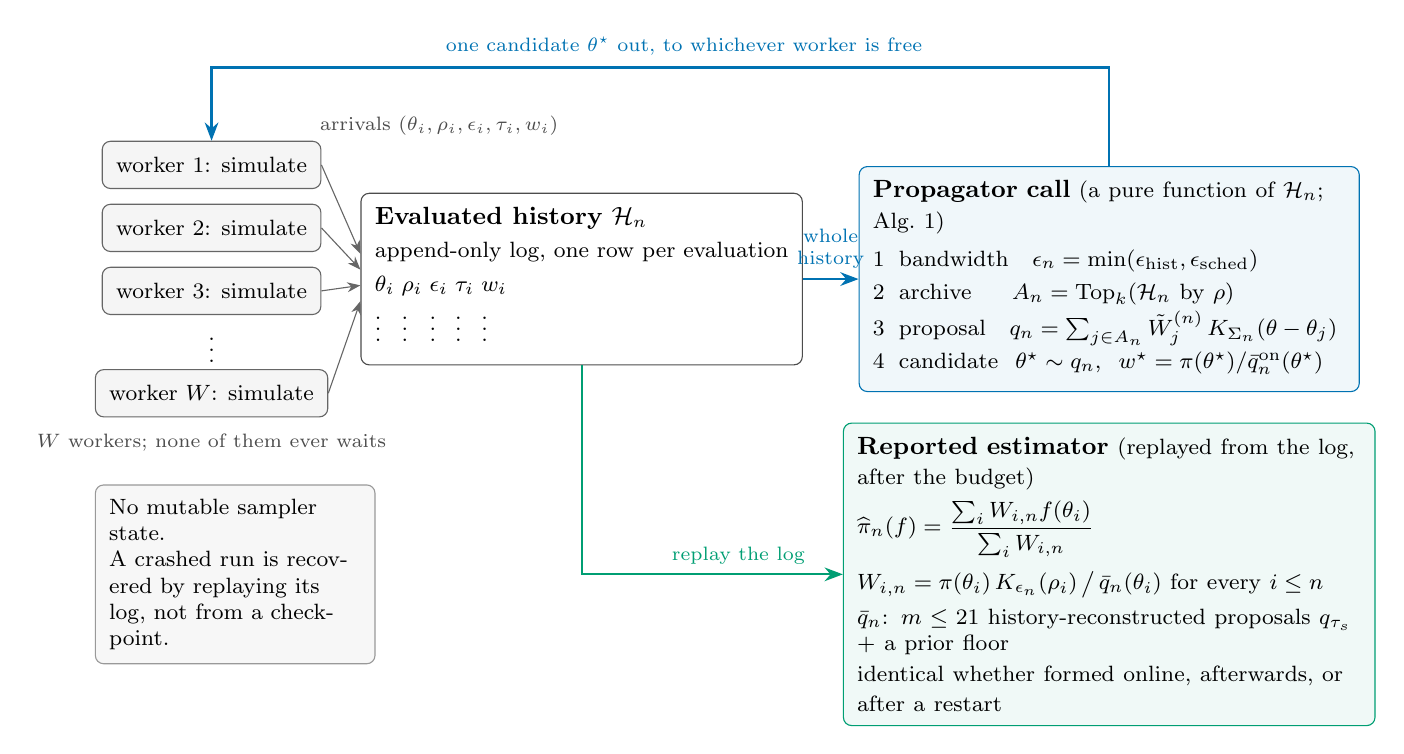
\begin{tikzpicture}[font=\small,>=Stealth,
  box/.style={draw,rounded corners=3pt,inner sep=5pt,align=left},
  lab/.style={font=\scriptsize,text=black!70,align=center}]

%% workers
\foreach \i/\y in {1/1.2,2/0.4,3/-0.4} {
  \node[box,draw=black!60,fill=black!4,minimum width=2.2cm,minimum height=0.6cm,font=\footnotesize] (w\i) at (0,\y) {worker \i: simulate};
}
\node[font=\footnotesize] at (0,-1.05) {$\vdots$};
\node[box,draw=black!60,fill=black!4,minimum width=2.2cm,minimum height=0.6cm,font=\footnotesize] (wW) at (0,-1.7) {worker $W$: simulate};
\node[lab,anchor=north] at (0,-2.1) {$W$ workers; none of them ever waits};

%% history log
\node[box,draw=black!70,fill=white,minimum width=3.3cm,align=left] (hist) at (4.7,-0.25) {%
  \textbf{Evaluated history} $\mathcal H_n$\\[1pt]
  {\footnotesize append-only log, one row per evaluation}\\[2pt]
  \begin{tabular}{@{}l@{\;}l@{\;}l@{\;}l@{\;}l@{}}
  \footnotesize$\theta_i$ & \footnotesize$\rho_i$ & \footnotesize$\epsilon_i$ & \footnotesize$\tau_i$ & \footnotesize$w_i$\\
  \footnotesize$\vdots$ & \footnotesize$\vdots$ & \footnotesize$\vdots$ & \footnotesize$\vdots$ & \footnotesize$\vdots$\\
  \end{tabular}};

%% propagator
\node[box,draw=async,fill=async!6,text width=6.0cm] (prop) at (11.4,-0.25) {%
  \textbf{Propagator call} {\footnotesize (a pure function of $\mathcal H_n$; Alg.~1)}\\[3pt]
  \begin{tabular}{@{}r@{\;\;}l@{}}
  \footnotesize 1 & \footnotesize bandwidth\quad $\epsilon_n=\min(\epsilon_{\text{hist}},\epsilon_{\text{sched}})$\\[1pt]
  \footnotesize 2 & \footnotesize archive\quad\ \ $A_n=\mathrm{Top}_k(\mathcal H_n\ \text{by}\ \rho)$\\[1pt]
  \footnotesize 3 & \footnotesize proposal\quad $q_n=\sum_{j\in A_n}\tilde W^{(n)}_j\,K_{\Sigma_n}(\theta-\theta_j)$\\[1pt]
  \footnotesize 4 & \footnotesize candidate\ \ $\theta^\star\sim q_n$,\ \ $w^\star=\pi(\theta^\star)/\bar q^{\mathrm{on}}_n(\theta^\star)$\\
  \end{tabular}};

%% reported estimator
\node[box,draw=reject,fill=reject!6,text width=6.4cm] (rep) at (11.4,-4.0) {%
  \textbf{Reported estimator} {\footnotesize (replayed from the log, after the budget)}\\[3pt]
  \footnotesize $\widehat\pi_n(f)=\dfrac{\sum_i W_{i,n}f(\theta_i)}{\sum_i W_{i,n}}$\\[4pt]
  \footnotesize $W_{i,n}=\pi(\theta_i)\,K_{\epsilon_n}(\rho_i)\,\big/\,\bar q_n(\theta_i)$ for every $i\le n$\\[3pt]
  \footnotesize $\bar q_n$: $m\le 21$ history-reconstructed proposals $q_{\tau_s}$ + a prior floor\\
  \footnotesize identical whether formed online, afterwards, or after a restart};

%% side note
\node[box,draw=black!40,fill=black!3,text width=3.2cm,font=\footnotesize,align=left] (note) at (0.3,-4.0)
  {No mutable sampler state.\\ A crashed run is recovered by replaying its log, not from a checkpoint.};

%% arrows
\foreach \i/\dy in {1/0.32,2/0.12,3/-0.08,W/-0.28} { \draw[->,black!60] (w\i.east) -- ($(hist.west)+(0,\dy)$); }
\node[lab,anchor=south west] at (1.25,1.45) {arrivals $(\theta_i,\rho_i,\epsilon_i,\tau_i,w_i)$};
\draw[->,async,thick] (hist.east) -- (prop.west) node[midway,above,lab,text=async] {whole\\history};
\draw[->,async,thick] (prop.north) -- ++(0,1.25) -| (w1.north);
\node[lab,text=async,anchor=south] at ($(prop.north)+(-5.4,1.28)$) {one candidate $\theta^\star$ out, to whichever worker is free};
\draw[->,reject,thick] (hist.south) |- (rep.west) node[pos=0.8,above,lab,text=reject] {replay the log};
\end{tikzpicture}
\end{document}
